% Template for a Computer Science Tripos Part II project dissertation
\documentclass[12pt,a4paper,twoside,openright]{report}
\usepackage[pdfborder={0 0 0}]{hyperref}    % turns references into hyperlinks
\usepackage[margin=25mm]{geometry}  % adjusts page layout
\usepackage{graphicx}  % allows inclusion of PDF, PNG and JPG images
%\usepackage{verbatim}
\usepackage{fancyvrb}
\VerbatimFootnotes
\usepackage{amsfonts}
\usepackage{amsmath}
\usepackage{minted}    % used for highlighted code fragments
\newminted{python}{frame=single,framesep=10pt,samepage}
\newminted{java}{frame=single,framesep=10pt,samepage}
\usepackage{docmute}   % only needed to allow inclusion of proposal.tex

\raggedbottom                           % try to avoid widows and orphans
\sloppy
\clubpenalty1000%
\widowpenalty1000%

\renewcommand{\baselinestretch}{1.1}    % adjust line spacing to make
% more readable

\begin{document}
\bibliographystyle{plain}

% Title

\pagestyle{empty}

\rightline{\LARGE \textbf{Jun Siang Cheah}}

\vspace*{60mm}
\begin{center}
	\Huge
	\textbf{An implementation and evaluation of Loopix, an anonymous communication system} \\[5mm]
	Computer Science Tripos -- Part II \\[5mm]
	Christ's College \\[5mm]
	\today  % today's date
\end{center}

%%%%%%%%%%%%%%%%%%%%%%%%%%%%%%%%%%%%%%%%%%%%%%%%%%%%%%%%%%%%%%%%%%%%%%%%%%%%%%
% Proforma, table of contents and list of figures

\pagestyle{plain}

\chapter*{Proforma}

{\large
	\begin{tabular}{ll}
		Name:               & \bf Jun Siang Cheah                               \\
		College:            & \bf Christ's College                              \\
		Project Title:      & \bf An implementation and evaluation of Loopix,   \\ 
		& \bf an anonymous communication system             \\
		Examination:        & \bf Computer Science Tripos -- Part II, July 2018 \\
		Word Count:         & \bf ???                                           \\
		Project Originator: & Dr Alastair Beresford                             \\
		Supervisor:         & Dr Alastair Beresford                             \\ 
	\end{tabular}
}
\footnotetext[1]{This word count was computed
	by \texttt{detex diss.tex | tr -cd '0-9A-Za-z $\tt\backslash$n' | wc -w}
}
\stepcounter{footnote}


\section*{Original Aims of the Project}


\section*{Work Completed}


\section*{Special Difficulties}

\newpage
\section*{Declaration}

I, Jun Siang Cheah of Christ's College, being a candidate for Part II of the Computer
Science Tripos, hereby declare that this dissertation and the work described in it are my own work,
unaided except as may be specified below, and that the dissertation
does not contain material that has already been used to any substantial
extent for a comparable purpose.

\bigskip
\leftline{Signed [signature]}

\medskip
\leftline{Date [date]}

\tableofcontents

%	\listoffigures

\newpage
\section*{Acknowledgements}

%%%%%%%%%%%%%%%%%%%%%%%%%%%%%%%%%%%%%%%%%%%%%%%%%%%%%%%%%%%%%%%%%%%%%%%
% now for the chapters

% Professional Practice & Presentation  14%
% Introduction and Preparation          26%
% Implementation	                    40%
% Evaluation and Conclusions	        20%


\pagestyle{headings}

\chapter{Introduction}

% The Introduction should explain the principal motivation for the project. Show how the work fits into the broad 
% area of surrounding Computer Science and give a brief survey of previous related work. It should generally be 
% unnecessary to quote at length from technical papers or textbooks. If a simple bibliographic reference is 
% insufficient, consign any lengthy quotation to an appendix.

% ~500 words

\section{Motivation}

Edward Snowden, Tor vuln to traffic analysis

\section{Overview}

\section{Related Work}

\subsection{Mix Networks and Onion Routing}

% ------INTRODUCTION END----------

\chapter{Preparation (Due 20th April)}

% Principally, this chapter should describe the work which was undertaken before code was written, hardware built
% or theories worked on. It should show how the project proposal was further refined and clarified, so that the
% Implementation stage could go smoothly rather than by trial and error.

% Throughout this chapter and indeed the whole dissertation, it is essential to demonstrate that a proper 
% professional approach was employed.

% The nature of this chapter will vary greatly from one dissertation to another but, underlining the professional 
% approach, this chapter will very likely include a section headed “Requirements Analysis” and incorporate other 
% references to software engineering techniques.

% The chapter will cite any new programming languages and systems which had to be learnt and will mention 
% complicated theories or algorithms which required understanding.

% It is essential to declare the Starting Point (see Section 7). This states any existing codebase or materials 
% that your project builds on. The text here can commonly be identical to the text in your proposal, but it may 
% enlarge on it or report variations. For instance, the true starting point may have turned out to be different 
% from that declared in the proposal and such discrepancies must be explained.

% ~2500 words

This chapter begins by providing a high level overview of how Loopix is structured, ......

\section{Structure of Loopix (Due 23rd March)}

In this section, I describe the Loopix network architecture, and the Poisson Mix theory. An overview of the network architecture is shown in Figure~\ref{fig:loopix_network}. 

\subsection{Network Architecture}

\begin{figure}[h]
	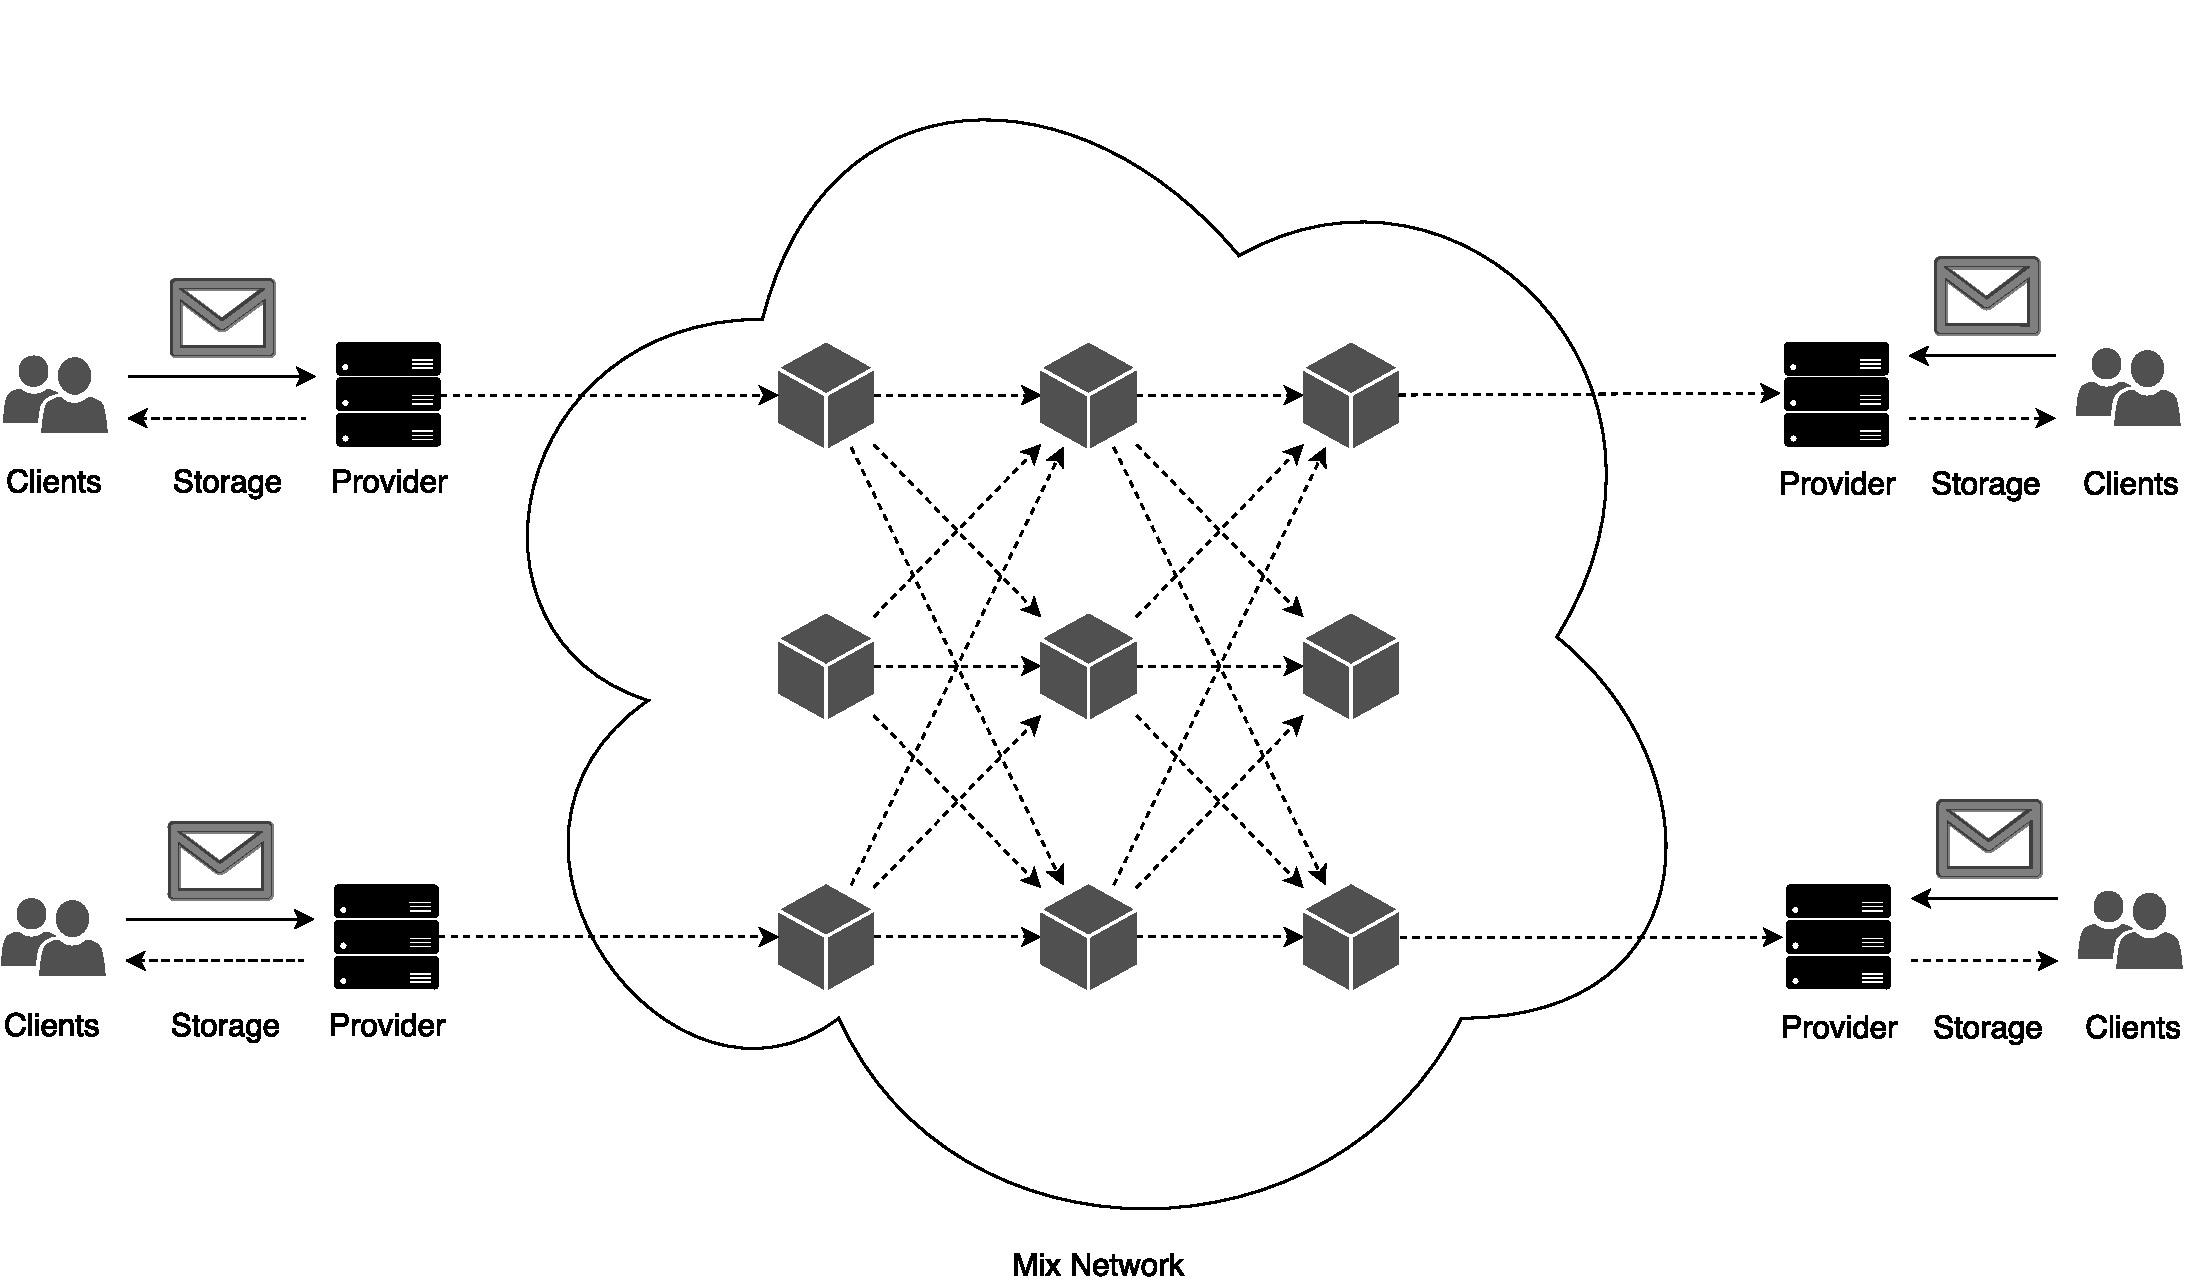
\includegraphics[width=\linewidth]{figs/loopix_network}
	\caption{Overview of the Loopix network architecture. Clients pass messages to their providers, which are responsible for injecting the message into the mix network. The received messages are stored in inboxes at providers and retrieved by clients when they come online. TODO: Refine the figure with message paths }\label{fig:loopix_network}
\end{figure}

The Loopix network is composed of three parts: clients, mix nodes and providers. A client can communicate through the Loopix network and can act as a sender and receiver of messages. Each entity in the Loopix network has a unique public-private key pair that is used to encrypt and decrypt messages. The mix nodes are separated into layers, with each layer forwarding messages to the next layer. 

In order for a sender to send a message to a receiver, the sender needs to know the receiver's Loopix network location, that is the IP address of the receiver's provider, an identifier of the user, and the receiver's public encryption key. The sender also needs to know the network locations of intermediate mix nodes as the sender is responsible for selecting the route through the network.


\subsection{Poisson Mix}

Loopix employs a strategy called the Poisson Mix to prevent observers from learning the correspondences between incoming and outgoing messages at a node, therefore guarding against a global passive adversary performing traffic analysis attacks. 

When a mix packet arrives at a mix node, the mix node decodes and extracts the subsequent mix packet to forward on. The decoded message includes a delay parameter which specifies how long to delay the forwarding of the packet. This delay parameter is determined by the source of the message. Honest clients choose this delay by sampling from an exponential distribution with a parameter $\lambda$ that is assumed to be public and the same for all mix nodes.

Since honest nodes generate cover traffic, loop traffic, and real traffic following a Poisson process, aggregating these traffic streams at the input of a mix node produces another Poisson process with a rate $\lambda_m$ dependent on the number of mix nodes and clients.

As this input process is a Poisson process, and each message is independently delayed using an exponential distribution with parameter $\lambda$, a Poisson Mix can be modelled as an $M/M/\infty$ queueing system since both input and output of the mix node are Poisson processes. As a result of the memoryless property of such a system, messages are indistinguishable from each other, since messages are emitted with equal probability regardless of the amount of time they have been waiting in the queue.

\section{Cryptography}

\subsection{Elliptic Curves}

\subsection{LIONESS Wide Cipher}

\section{Requirements Analysis}

Sphinx, Loopix, Testnet, Evaluation

\section{Development Tools}

IDEA IntelliJ

Docker

\section{Existing Libraries}

\subsection{Python Loopix Library}

\subsection{Bouncy Castle}

Crypto (AES/SHA/HMAC/ECC)

Chosen for easier portability between clients which may not have the official java crypto extension installed, or have the neccessary ciphers.

\section{Software Engineering Techniques}

Test driven development. Existing library allows generation of test data to verify correctness and compatibility.

% --------PREPARATION END--------------

\chapter{Implementation (Due 6th April)}

% This chapter should describe what was actually produced: the programs which were written, the hardware which was
% built or the theory which was developed. Any design strategies that looked ahead to the testing stage might 
% profitably be referred to (the professional approach again).

% Descriptions of programs may include fragments of high-level code but large chunks of code are usually best left % to appendices or omitted altogether. Analogous advice applies to circuit diagrams.
% Draw attention to the parts of the work which are not your own. Making effective use of powerful tools and 
% pre-existing code is often laudable, and will count to your credit if properly reported.
% It should not be necessary to give a day-by-day account of the progress of the work but major milestones may 
% sometimes be highlighted with advantage.

% ~4500 words

In this chapter, I will describe how I implemented my project, describing challenges faced along the way. The implementation consists of the following:

\begin{itemize}
	\item A library for creating and processing Sphinx packets
	\item A library for sending and receiving messages on the Loopix network
	\item A command-line chat client that broadcasts messages to all clients on the network
	\item A testing framework for starting a test network
\end{itemize}

As Loopix uses the Sphinx packet format, I have implemented my own Java library of Sphinx. As such, the project is split into two libraries, with the low level cryptographic elements and packet format implemented in Sphinx, and the high-level network decisions such as path selection and routing implemented in Loopix. The Loopix library provides a basic event-driven API for sending and receiving messages.

\section{Sphinx Library}

The Sphinx library provides an API for creating and processing Sphinx packets as generated by the \verb|sphinxmix| Python package, and is based heavily on the package. This distinction is necessary to meet the project goal of binary compatibility with the existing Python Loopix implementation. \verb|sphinxmix|'s implementation deviates in several places when compared with the algorithm described in the Sphinx paper.

\subsection{Sphinx Parameters}

The \verb|SphinxParams| class encapsulates all of the cryptography and the various parameters for a Sphinx packet, such as the security parameter (key size), header size, body size, various hash functions, and the LIONESS wide block cipher.

AES, SHA256, LIONESS, HMAC-SHA256

\subsection{Packet Creation}

Each Sphinx packet consists of two parts, the header and the body. The header contains information to correctly process the packet, and the body contains the encrypted payload. The packet has the following structure:

\begin{javacode}
public class SphinxPacket {
	public SphinxHeader header;
	public byte[] body;
}
\end{javacode}
	
\subsubsection{Sphinx Packet Header}

The header has the following structure:

\begin{javacode}
public class SphinxHeader {
	public ECPoint alpha;
	public byte[] beta;
	public byte[] gamma;
}
\end{javacode}

\begin{itemize}
	\item \verb|alpha| is an elliptic curve group element ($\alpha = g^b$) used to derive the per-hop shared secret required to authenticate and process the rest of \verb|SphinxHeader|. It is also used to decrypt a layer of the Sphinx body payload.
	\item \verb|beta| is a list of per-hop routing data and padding that is encrypted in a nested manner. Each layer contains routing commands that is defined and processed by a Sphinx node.
	\item \verb|gamma| is a HMAC-SHA256 message authentication code tag that covers \verb|alpha| and \verb|beta|
\end{itemize}

Header creation is handled in the \verb|SphinxClient| class. Header creation takes as input a sequence of mix nodes $\{n_0,..,n_{\nu-1}\}$ and their corresponding public keys $\{y_0,...,y_{\nu-1}\}$, and outputs a \verb|SphinxHeader| object and a list of per-hop shared secrets $\{s_0,...,s_{\nu-1}\}$. The function signature is given below.

\begin{javacode}
private static SphinxHeaderData createHeader(SphinxParams params,
	List<byte[]> path,
	List<ECPoint> keys,
	byte[] destination) throws CryptoException
\end{javacode}

Header creation first starts with the derivation of key material for each hop. This key material will be used to encrypt and authenticate the rest of the header, and the packet payload. Initially, a random $b \in_R \mathbb{Z}^*_q$ is chosen. This will be used as the initial blinding factor. A sequence of $\nu$ tuples $(\alpha_0, s_0, b_0),...,(\alpha_{\nu-1}, s_{\nu-1}, b_{\nu-1})$ is computed as follows:
\\
\begin{itemize}
	\setlength\itemsep{-0.4em}
	\item $\alpha_0 = g^b, s_0 = y_0^b, b_0 = h_b(s_0)*b$
	\item $\alpha_1 = g^{b_0}, s_1 = y_1^{b_0}, b_1 = h_b(s_1)*b_0$
	\item ...
\end{itemize}

\begin{itemize}
	\item $\alpha_n$ is the group element used in the Ephemeral Elliptic-curve Diffie-Hellman key exchange (ECDHE) to generate a shared secret. $\alpha_n$ can be thought of as an ephemeral public key. 
	%$\alpha_n$ is the exponentiation of the group generator $g$ with a blinding factor $b_{n-1}$. 
	
	\item $s_n$ is the shared secret for hop $n$. 
	%$s_n$ is the exponentiation of the hop's public key $x_n$ with the blinding factor $b_{n-1}$, that is $s_n = x^{b_{n-1}}_n$. 
	As the public key $y_n$ is of the form $g^{x_n}$, $s_n = (g^{x_n})^{b_{n-1}} = g^{{x_n}{b_{n-1}}}$. The shared secret is then passed into a key derivation function to produce an AES encryption key. The key derivation is done by passing the binary representation of the shared secret into the SHA-256 hash function and truncating the output to the security parameter $\kappa$.
	
	\item $b_n$, the blinding factor to be used for the next hop. This is computed by passing $s_n$ into a hash function $h_b$, which is implemented by using $s_n$ as an AES encryption key and encrypting a block of all zeroes. \footnote{The \verb|sphinxmix| package deviates from the paper here as the paper describes $b_n = h_b(\alpha_n, s_n)$, but the actual implementation ignores $\alpha_n$ and does $b_n = h_b(s_n)$.}
\end{itemize}


At the end of this derivation process, a list of $(\alpha_n, s_n, b_n)$ tuples, each corresponding to a hop in the path is generated. \verb|header.alpha| is set as $\alpha_0$.

The next step is to generate filler strings $\phi_i$ that serves as encrypted padding for $\beta$, routing information block. This is done by repeatedly encrypting the padding block with each hop's shared secret.

|possibly add phi diagram|

$\beta$ and $\gamma$ are generated next. Starting from the terminal hop, a sequence of headers $M_{\nu-1},M_{\nu-2},...,M_{0}$, where $M_i = (\alpha_i, \beta_i, \gamma_i)$ is computed as follows:

\begin{itemize}
	\setlength\itemsep{-0em}
	\item $\beta_{\nu-1} = \rho(h_\rho(s_{\nu-1}), \{{\text{destination-identifier}}\|\phi_{\nu-1}\})_{[0..\text{header size}]}$
	\item $\beta_{i} = \rho(h_\rho(s_{i}), \{n_{i+1} \| \gamma_{i+1} \| \beta_{i+1}\})_{[0..\text{header size}]}$ for $0 \le i < \nu - 1$
	\item $\gamma_i = \mu(h_\mu(s_{i}), \beta_i)$
\end{itemize}

\begin{itemize}
	\item $\rho$ is implemented using AES-128-CTR.
	\item $h_\rho$ is a hash function implemented using AES-128-CTR, by encrypting the string \verb|hrhohrhohrhohrho| using the parameter to $h_\rho$ as the encryption key.
	\item $\mu$ is implemented using HMAC-SHA256.
	\item $h_\mu$ is a hash function implemented using AES-128-CTR, by encrypting the string \verb|hmu:hmu:hmu:hmu:| using the parameter to $h_\mu$ as the encryption key.
	\item $\beta_i$ consists of either the destination identifier and the encrypted padding $\phi_{\nu-1}$, or a routing command $n_{i+1}$, a MAC $\gamma_{i+1}$ and a encrypted routing command block $\beta_{i+1}$ to forward to the next node.
\end{itemize}

\verb|header.gamma| is set to $\gamma_0$, and \verb|header.beta| is set to $\beta_0$. The final header structure when $\nu = 4$ is illustrated in Figure~\ref{fig:sphinx_header}. At the end of this process, a \verb|SphinxHeader| object with the necessary data $M_0$ and a list of per-hop shared secrets are created. The list of shared secrets will be later used for encrypting the payload.

|possibly add (beta, gamma) diagram|


\begin{figure}[h]
	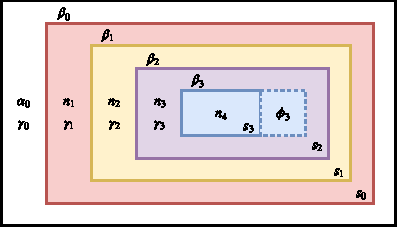
\includegraphics[width=\linewidth]{figs/sphinx_header}
	\caption{Sphinx header for a packet with 4 hops}\label{fig:sphinx_header}
\end{figure}

\subsubsection{Sphinx Forward Packet Body}

Body creation is handled in the \verb|SphinxClient| class.  The function signature for creating an entire \verb|SphinxPacket| is given below.

\begin{javacode}
public static SphinxPacket createForwardMessage(SphinxParams params,
	List<byte[]> path,
	List<ECPoint> keys,
	Value destination,
	byte[] message) throws SphinxException
\end{javacode}

\verb|createForwardMessage| takes as inputs a sequence of mix nodes and their corresponding public keys as per the header generation section above, and a message $m$ of type \verb|byte[]|. It performs the following operations:

\begin{enumerate}
	\item \verb|message| is concatenated with the destination identifier and serialised using \verb|msgpack|, then padded to a fixed size.
	\item A call is made to \verb|createHeader| to generate a \verb|SphinxHeader| and the list of shared secrets $\{s_0,...,s_{\nu-1}\}$ to encrypt \verb|message| with.
	\item Starting from the terminal hop, \verb|message| is repeated encrypted using $\pi$ with a key derived from the hop's shared secret. That is,
		\begin{itemize}
			\setlength\itemsep{-0em}
			\item $\delta_{\nu-1} = \pi(h_\pi(s_{\nu-1}), m)$
			\item $\delta_i = \pi(h_\pi(s_{i}), \delta_{i+1})$
		\end{itemize}
	and as implemented:
	\begin{javacode}
byte[] delta = paddedBody;
for (int i = path.size() - 1; i >= 0; i--) {
	delta = params.pi(
		params.hpi(header.keys.get(i)), 
		delta
	);
}
	\end{javacode}
\end{enumerate}

The output of this process is the tuple $(M_0, \delta_0)$, which should be forwarded to the mix node $n_0$.

\subsection{Packet Serialisation}

msgpack

\subsection{Packet Processing}

\subsection{Challenges Faced}

Most of the challenges faced involves differences in language support for certain features between Java and Python.

There were a lot of byte array manipulations that primarily involved slicing arrays into different pieces, which is easily done in Python. However, in Java this caused the code to be very verbose and very hard to read.

The structure of how data is passed around also introduced readability issues, as the original implement made good use of tuple return types, which meant the creation of a lot of different classes in the Java codebase.

\section{Loopix Client Library}

\subsection{Public Key Infrastructure}

sqlite db

\subsection{Path Selection}

random selection, delay sampling

\section{Chat Client}

\section{Testing Framework}

\subsection{Unit Tests}

JUnit

\subsection{Continuous Integration}

Travis.CI (should this be under software engineering techniques in prep?)

\subsection{Docker Containers}

\section{Challenges Faced}

% ---------IMPLEMENTATION END---------------

\chapter{Evaluation (Due 13th April)}

% This is where Assessors will be looking for signs of success and for evidence of thorough and systematic 
% evaluation as discussed in Section 8.3. Sample output, tables of timings and photographs of workstation screens,
% oscilloscope traces or circuit boards may be included. A graph that does not indicate confidence intervals will 
% generally leave a professional scientist with a negative impression.

% As with code, voluminous examples of sample output are usually best left to appendices or omitted altogether.
% There are some obvious questions which this chapter will address. How many of the original goals were achieved? 
% Were they proved to have been achieved? Did the program, hardware, or theory really work?
% Assessors are well aware that large programs will very likely include some residual bugs. It should always be 
% possible to demonstrate that a program works in simple cases and it is instructive to demonstrate how close it 
% is to working in a really ambitious case.

% ~2000 words

\section{Functional Testing}

\section{Performance}

\section{Viability on Mobile Devices}

\section{Security Evaluation}

% -----------EVALUATION END--------------------

\chapter{Conclusion}

% This chapter is likely to be very short and it may well refer back to the Introduction. It might properly explain how you would have planned the project if starting again with the benefit of hindsight.

% ~500 words

%%%%%%%%%%%%%%%%%%%%%%%%%%%%%%%%%%%%%%%%%%%%%%%%%%%%%%%%%%%%%%%%%%%%%
% the bibliography
\addcontentsline{toc}{chapter}{Bibliography}
\bibliography{refs}

%%%%%%%%%%%%%%%%%%%%%%%%%%%%%%%%%%%%%%%%%%%%%%%%%%%%%%%%%%%%%%%%%%%%%
% the appendices
\appendix

\chapter{Project Proposal}

%% Note: this file can be compiled on its own, but is also included by
% diss.tex (using the docmute.sty package to ignore the preamble)
\documentclass[12pt,a4paper,twoside]{article}
\usepackage[pdfborder={0 0 0}]{hyperref}
\usepackage[margin=25mm]{geometry}
\usepackage{graphicx}
\usepackage{parskip}
\begin{document}
	
	\begin{center}
		\Large
		Computer Science Tripos -- Part II -- Project Proposal\\[4mm]
		\LARGE
		An implementation and evaluation of Loopix, an anonymous communication system\\[4mm]
		
		\large
		Jun Siang Cheah, Christ's College
		
		Originator: Dr Alastair Beresford
		
		19 October 2017
	\end{center}
	
	\vspace{5mm}
	
	\textbf{Project Supervisor:} Dr Alastair Beresford
	
	\textbf{Director of Studies:} Dr Richard Mortier
	
	\textbf{Project Overseers:} Dr Timothy Jones \& Prof Marcelo Fiore 
	
	% Main document
	
	\section*{Introduction}
	
	Anonymous communication systems such as Tor are becoming increasingly important in the current age of pervasive data collection, surveillance and censorship, allowing for privacy and anonymity when parties are trying to collect as much data as possible on individuals, either for commercial exploitation or government surveillance.
	
	However, the most widely used anonymous communication system, Tor, is vulnerable to attacks such as traffic correlation by a global passive adversary and corrupt nodes performing active attacks to deanonymise users. Government agencies such as the National Security Agency (NSA) and Government Communications Headquarters (GCHQ) have already demonstrated the ability to deanonymise a small fraction of Tor users.\cite{torstinks} Alternative systems that are not vulnerable to a global passive adversary tend to be high-latency, low-bandwidth, which severely limits possible applications.
	
	Loopix\cite{piotrowska2017loopix} is a newly proposed protocol that provides medium-latency, low-bandwidth communication that provides strong anonymity against both active attackers and global passive adversaries. The medium-latency property of the system allows for both low-latency applications such as instant messaging and high-latency applications such as email. Another feature of Loopix is the ability to store messages for offline clients. This is helpful for peer-to-peer communications when it is difficult to have both clients online at the same time such as mobile devices.
	
	Currently, the reference proof of concept implementation is written in Python with a dependency on Sphinx\cite{danezis2009sphinx}. A Python implementation works well enough for server nodes where there are not many constraints, however, the Python code is not portable for mobile devices. As such, I plan to implement Loopix as a Java library, which can then run on any system with a JVM installed such as Android. After the implementation is complete, I would evaluate the performance of the system (bandwidth, latency, and complexity) and validate some of the privacy claims in the original paper.
	
	
	\section*{Starting point}
	
	%\emph{Describe existing state of the art, previous work in this area,
	%  libraries and databases to be used. Describe the state of any
	%  existing codebase that is to be built on.}
	
	Currently, there exists a Python implementation of Loopix which I plan to use to test my own implementation against and would allow for a faster iteration cycle as I wouldn't need a complete implementation to begin testing. I will also refer to the existing implementation for details that are specified in the paper. I will also rely on the BouncyCastle Java library for cryptographic primitives.
	
	The cryptography used will relate to the Security I and II courses, and I will draw upon the Part IB Mathematical Methods course for the statistical theory used in Loopix. I have some experience with the theory behind mix networks from working with Tor.
	
	I have written an existing Android application that currently uses Tor for peer-to-peer communication which can be adapted to use Loopix instead for demonstration purposes.
	
	\section*{Project structure}
	
	The aim of this project is to provide a Java library implementation of Loopix, therefore taking advantage of the ubiquity of JVMs to run Loopix on a larger range of devices, with a primary goal of allowing Android applications to use Loopix for communication.
	
	The project can be broken down into the following sub-projects:
	
	\begin{enumerate}
		\item \textbf{Implementation of the Sphinx library:} Loopix uses the Sphinx mix format as the interchange format for messages, thus a Java Sphinx library needs to be written before any work on Loopix can proceed. Sphinx uses AES, Diffie-Hellman and SHA256 cryptographic primitives, which are implemented by the BouncyCastle library. I will use the existing implementation to test my own implementation by generating and parsing messages on both sides.
		\item \textbf{Implementation of the Loopix library:} This library will the at the very minimum provide a client implementation of Loopix that is compatible with the existing Python implementation for servers. The Loopix architecture calls for 3 components: the client, provider and mix nodes. All 3 share the same message processing pipeline and only differ in behaviour upon parsing the decrypted message.
		\item \textbf{Demonstration application:} An application that uses the resulting Java library to demonstrate that the library is working. A possible application to implement is an instant messaging application.
		\item \textbf{Evaluation:} The final part of the project is to benchmark the performance of the implementation in terms of bandwidth and latency overheads. I will also need to verify some of the claims made in the paper.
	\end{enumerate}
	
	\section*{Success criteria}
	
	The project will be a success if:
	
	\begin{itemize}
		\item I have completed a Java implementation of the Sphinx library.
		\item I have completed at the very minimum a client implementation of Loopix in Java.
		\item I have created a demo app that uses the library to send messages.
		\item I have produced an evaluation of my Loopix implementation, in terms of bandwidth throughput, bandwidth overhead, latency overhead, complexity overhead and privacy metrics.
	\end{itemize}
	
	
	\section*{Possible extensions}
	
	If I achieve my main result early, then possible extensions include:
	
	\begin{itemize}
		\item \textbf{Discoverability:} At the moment, all nodes in the network must be preloaded with a list of all the other nodes in the network, including their IP address and public keys. This simply does not scale and fails to deal with failures with some of the nodes in the network and mobility of real clients. A potential solution could be to borrow Tor's directory authority model and implement it within Loopix. Implementing a directory also allows for a scheme similar to Tor's .onion domain names to refer to other nodes, rather than their IP address.
		\item \textbf{Provider resource starvation:} Currently, providers store all messages in memory with no eviction strategy. This is bad in many ways, as providers can run out of memory due to either a malicious actor flooding the provider with messages, an organic increase in traffic or users never coming online to clear their inbox. I could research into methods for mitigating and handling this issue, as a user would find messages disappearing a bad experience.
		\item \textbf{Android application demo:} I could build a demo app on Android which is where Loopix shines with its offline message storage.
	\end{itemize}
	
	
	\section*{Timetable and milestones}
	
	\textbf{Weeks 1-2 | 16 Oct - 29 Oct | Michaelmas term}
	
	\begin{itemize}
		\item Familiarise myself with the Sphinx and Loopix papers and implementation.
		\item Setup test scripts for comparing outputs from Sphinx/Loopix.
	\end{itemize}
	
	\textbf{Weeks 3-4 | 30 Oct - 12 Nov | Michaelmas term}
	
	\begin{itemize}
		\item Implement the Sphinx library in Java.
	\end{itemize}
	
	\textbf{Milestone 1: }Sphinx library completed
	
	\textbf{Weeks 5-8 | 13 Nov - 17 Dec | Michaelmas term + Christmas vacation}
	
	\begin{itemize}
		\item Implement the client portion of the Loopix library in Java.
		\item Create a command line wrapper around the library to test with.
		\item Start initial testing using the existing Python implementation to setup providers and mix nodes on a small scale.
	\end{itemize}
	
	\textbf{Milestone 2:} Client portion of the library done, and I can send and receive messages using the library.
	
	\textbf{Weeks 9-10 | 18 Dec - 31 Dec | Christmas vacation}
	
	\begin{itemize}
		\item Implement the provider/mix node portion of the Loopix library.
	\end{itemize}
	
	\textbf{Weeks 11-13 | 1 Jan - 21 Jan | Christmas vacation + Lent term}
	
	Contingency time set aside for any major issues found up to this point.
	
	\textbf{Weeks 14-15 | 22 Jan - 4 Feb | Lent term}
	
	\begin{itemize}
		\item Implement a demo application that uses the Loopix library.
		\item Submit Progress Report
	\end{itemize}
	
	\textbf{Milestone 3:} A working demo that can be shown to my supervisor/DoS.
	
	\textbf{Weeks 16-17 | 5 Feb - 18 Feb | Lent term}
	
	\begin{itemize}
		\item Research existing attacks on anonymous communication systems.
	\end{itemize}
	
	\textbf{Weeks 18-20 | 19 Feb - 11 Mar | Lent term}
	
	\begin{itemize}
		\item Evaluate the project, recording any necessary data.
	\end{itemize}
	
	\textbf{Milestone 4:} Evaluation data gathered
	
	\textbf{Weeks 21-25 | 12 Mar - 15 Apr | Lent term + Easter vacation}
	
	\begin{itemize}
		\item Write and submit my draft dissertation.
	\end{itemize}
	
	\textbf{Milestone 5:} Draft dissertation complete!
	
	\section*{Resources required}
	
	A list of required resources:
	
	\begin{itemize}
		\item My own machines:
		\begin{itemize}
			\item Desktop computer (AMD Ryzen 5 1600, 32GB RAM, Windows/Ubuntu 16.04)
			\item Laptop (Intel i7-4720HQ, 8GB RAM, Windows)
			\item Backup desktop (Intel i5-6500, 16GB RAM, Windows/Ubuntu 16.04)
		\end{itemize}
		\item My own dedicated servers (2x Intel i5-2300, 16GB RAM, Ubuntu 16.04)
		\item BouncyCastle library\footnote{\url{https://www.bouncycastle.org/}}
		\item Loopix source\footnote{\url{https://github.com/UCL-InfoSec/loopix}}
	\end{itemize}
	
	Backups will be provided by Dropbox and OneDrive. Revision control will be provided using GitHub, with a backup remote on Bitbucket. I can switch to using the MCS machines if my personal machines fail, and use student credit to run VMs with cloud providers if my servers fail.
	
	\bibliographystyle{unsrt}
	\bibliography{refs}
	
\end{document}


\end{document}